\documentclass[conference]{IEEEtran}
\IEEEoverridecommandlockouts
\usepackage{amsmath,amssymb,amsfonts}
\usepackage{graphicx}
\usepackage{booktabs}
\usepackage{multirow}
\usepackage{array}
\usepackage{xcolor}
\usepackage{tikz}
\usetikzlibrary{arrows.meta,positioning,fit,calc,shapes.geometric}
\usepackage[hidelinks]{hyperref}
\usepackage{cite}

\definecolor{cblue}{HTML}{2a78d6}
\definecolor{corange}{HTML}{eb6834}
\definecolor{caqua}{HTML}{1baf7a}
\definecolor{cink}{HTML}{52514e}
\newcommand{\BA}{\textrm{BA}}
\newcommand{\MA}{\textrm{MA}}
\newcommand{\code}[1]{\texttt{\small #1}}

\begin{document}

\title{Malicious Forgetting Meets Zero Knowledge:\\
Reproducing the FUsion Backdoor in Active Federated Unlearning\\
and Preventing It with Verifiable Groth16 Training Proofs}

\author{}

\maketitle

\begin{abstract}
Active federated unlearning (FU) lets clients ask a federation to forget part of their data, and it
trusts them to run the unlearning honestly. The FUsion backdoor (INFOCOM 2026) abuses that trust:
malicious clients behave honestly during training, secretly prepare a compact backdoor subnetwork,
request unlearning, and fuse the subnetwork into their unlearning updates. We first reproduce
FUsion and its statistical defence, SubID, end to end. On MNIST, the backdoor reaches
$\BA=0.986$ while main-task accuracy is preserved, and SubID identifies both attackers with
$F_1=1.0$. We then implement the cryptographic prevention proposed in \emph{Verifiable Federated
Unlearning with Zero-Knowledge Proofs}. Every client update, in learning and in unlearning, must
carry a Groth16 proof that it is exactly one fixed-point SGD step of the model head. The step must
start from the server's model, use a server-chosen batch from a Merkle-committed dataset, and apply
a public per-sample forget mask. The circuit has 290\,129 R1CS constraints. A proof takes
$1.44\pm0.06$\,s on a laptop CPU, verification takes 1.8\,ms, and a proof is 196 bytes; the
fixed-point head is bit-identical to a native reference trainer on 1000 random steps. In a
50-client federation with 10 attackers, FUsion reaches $\BA=1.000$ without verification. Proving
every update rejects all attackers at their first patched round ($\BA=0.013$, no false positives).
Random auditing cuts proving cost by 80--95\,\% and still prevents the backdoor, but \emph{only} if
a detected cheat rolls the model back. Without rollback the attack succeeds ($\BA=0.789$). We also
find that FUsion needs only $m=6$ patched rounds in this setting rather than the $m=40$ assumed by
the auditing analysis, and we quantify the consequences.
\end{abstract}

\begin{IEEEkeywords}
Federated unlearning, backdoor attacks, zero-knowledge proofs, Groth16, verifiable training, gnark,
Poseidon2, random auditing.
\end{IEEEkeywords}

%=====================================================================
\section{Introduction}
%=====================================================================
Regulations such as the GDPR give individuals a \emph{right to be forgotten}~\cite{gdpr}. In federated
learning (FL)~\cite{fedavg}, this motivates \emph{federated unlearning} (FU): the influence of some
training data is removed from the global model without retraining from scratch. In \emph{active}
FU, the clients whose data is removed take part in the unlearning and run it on their own
machines~\cite{fusion}. The server never sees client data, so it must trust that each unlearning
update is honest.

Zhao et~al.~\cite{fusion} showed that this trust can be exploited. In their \emph{FUsion backdoor},
malicious clients send clean updates during training, which evades training-time defences. Offline,
they build a compact backdoor subnetwork. They then request unlearning and, in every unlearning
round, fuse that subnetwork into an otherwise legitimate unlearning update. Unlearning updates are
naturally noisy and heterogeneous, so the server cannot tell them apart. The same paper proposes
\emph{SubID}, a statistical detector based on subspace deviations.

A companion design~\cite{zkdesign} takes a cryptographic route. If every update must come with a
zero-knowledge proof that it is the output of a fixed, server-defined procedure applied to the
client's own committed data, then a patched update simply has no valid proof. This report
implements and evaluates both lines of work.

\textbf{Contributions.}
\begin{enumerate}
\item An end-to-end reproduction of FUsion (backdoor-critical layers, Grad-CAM trigger-sensitive
units, subnetwork fusion) and SubID on MNIST, with a cleartext \emph{replay oracle} that previews
the zero-knowledge guarantee (Part~I, \S\ref{sec:part1}).
\item A complete Groth16 implementation of the verifiable FL/FU design (Part~II): a fixed-point
training circuit with Poseidon2 Merkle commitments and a forget bitmask; a native trainer proved
bit-identical to the circuit; prover, verifier and server CLIs; and the paper's random-auditing
scheme (\S\ref{sec:design}--\S\ref{sec:impl}).
\item A justification of every design choice: why Groth16, why Poseidon2, why a frozen extractor
with a proved head, why MSE, the fixed-point bound derivation, and why the inputs are packed. Each
is backed by measurements (\S\ref{sec:why}, \S\ref{sec:circuit}).
\item A measured evaluation: constraint counts, the time of every pipeline step, accuracy cost of
fixed point, and attack-versus-defence outcomes with full and audited verification. It also yields
three findings that refine the design's claims (\S\ref{sec:eval}, \S\ref{sec:discussion}).
\end{enumerate}

%=====================================================================
\section{Background}
%=====================================================================
\subsection{Federated learning and active unlearning}
A server holds the global model $w_t$, sends it to $n$ clients, and aggregates their local updates
with FedAvg, $w_{t+1}=w_t+\frac1n\sum_i g_i^{t+1}$~\cite{fedavg}. Active FU optimises
\begin{equation}
\min_w\; \mathcal{L}(D_{\text{retain}};w)+\varphi\,R(w,w_T,D_{\text{unlearn}}),
\end{equation}
usually approximated by lightweight retraining or correction~\cite{fusion}. We use NoT
(Negation-of-Training)~\cite{not}, which negates selected layers of the converged model once and
then fine-tunes on retained data.

\subsection{The FUsion backdoor~\cite{fusion}}
Malicious clients $C_{\text{mal}}$ ($m<n/2$) own poisoned samples $(x',y_t)$ carrying a trigger.
\begin{itemize}
\item \emph{Preparation (during FL, never submitted).} Each attacker trains a local backdoor
model $g^{bd}_i$ on $\mathcal{L}_{\text{mal}}=\mathbb{E}_{D^c}[\mathcal{L}]+\gamma\,
\mathbb{E}_{D^p}[\mathcal{L}(w;x',y_t)]$.
\begin{itemize}
\item \emph{Backdoor-critical (BC) layers.} The attacker measures the backdoor-accuracy drop
$\Delta b_i(h)$ when layer $h$ of $g^{bd}_i$ is replaced by its benign counterpart, normalises it as
$\delta_i(h)=\Delta b_i(h)/\max_j\Delta b_i(j)$, and averages over attackers to get $\bar\delta(h)$.
It anchors at $h^*=\arg\max_h\bar\delta(h)$ and expands contiguously while
$\bar\delta(h)\ge\theta\,\bar\delta(h^*)$.
\item \emph{Trigger-sensitive (TS) units.} Grad-CAM~\cite{gradcam} scores rank the units inside the
BC layers, and the top-$\rho$ fraction is kept.
\item \emph{Subnetwork.} Only the TS units are trained, on
$\mathcal{L}_{\text{sub}}=\lambda_1\mathcal{L}(f_{H_{BC}}(z_{bd}),y_t)+\lambda_2\|f_{H_{BC}}(z_{\text{clean}})\|^2$,
which yields $S_{bd}$, non-zero only in the BC layers.
\end{itemize}
\item \emph{Injection (every FU round).} After legitimate unlearning, the attacker fuses
$\tilde w_i^t=\hat w_i^t+\beta S_{bd}$ and fine-tunes on
$\mathcal{L}_{\text{unlearn}}=\mathcal{L}(\text{clean})+\lambda\mathcal{L}(\text{backdoor})$. It then
submits $\tilde g_i^t=\tilde w^{t*}_i-\hat w_t$.
\end{itemize}

\subsection{SubID~\cite{fusion}}
The server stacks the client updates of the last $T_r$ training rounds into $G_{\text{train}}$. Its
top-$k$ left singular vectors span a benign subspace $S_{\text{benign}}$. In each unlearning window
of $\tau$ rounds, the server computes residuals $\delta_i^t=\hat g_i^t-P_{S_{\text{benign}}}(\hat g_i^t)$
and takes the top-$k$ singular vectors of the residuals as the deviation subspace $S^a_{\text{dev}}$.
Each client's score is $\phi^a_i=\|P_{S^a_{\text{dev}}}(\bar g_i)\|_2$, and the client is flagged if
$\phi_i^a>\text{median}+\kappa\cdot\text{MAD}$. A client flagged in more than a fraction $\phi$ of
windows is declared malicious.

\subsection{Zero-knowledge proofs and Groth16}
A zk-SNARK lets a prover convince a verifier that it knows a private witness $w$ such that
$C(x,w)=1$ for a public statement $x$. The proof reveals nothing beyond that fact and is short and
fast to check. Groth16~\cite{groth16} proves satisfiability of a rank-1 constraint system (R1CS),
$\langle a_k,z\rangle\cdot\langle b_k,z\rangle=\langle c_k,z\rangle$, over the scalar field of a
pairing-friendly curve. Its proof is three group elements and verification needs three pairings,
but it requires a circuit-specific trusted setup. Arithmetic is over a prime field
($p\approx2^{254}$ for BN254), so integers wrap modulo $p$. Range checks are therefore essential for
any circuit that emulates integer arithmetic.

%=====================================================================
\section{Threat Model}
%=====================================================================
There are $n$ clients and one honest-but-curious server, and all clients take part in every round.
Up to $m<n/2$ clients are controlled by an attacker who knows their data and can send arbitrary
updates, but cannot see benign clients' data or updates. The attacker's goal is a targeted backdoor
(trigger $\to$ label $y_t$) with main-task accuracy preserved. Training-time defences force the
attacker to stay honest during FL, so it attacks only through its unlearning updates. In Part~II
the attacker also knows the verification scheme and the audit probability, but not which rounds
will be audited. Poisoned samples placed in the committed dataset from the start count as ordinary
data poisoning, which is out of scope~\cite{zkdesign}.

%=====================================================================
\section{Part I: Reproducing FUsion and SubID}\label{sec:part1}
%=====================================================================
\textbf{Setup.}
\begin{itemize}
\item \emph{Model and data:} MNIST, a CNN with 47k parameters (conv--conv--fc--fc), 10 IID clients
of which 2 (20\,\%) are malicious.
\item \emph{Schedule:} 25 FedAvg rounds of FL, then 60 FU rounds with NoT.
\item \emph{Trigger:} a 3$\times$3 white square in the bottom-right corner, target label 0, with
10\,\% of each attacker's data poisoned.
\item \emph{FUsion hyperparameters (the paper's defaults):} $\theta=0.6$, $\rho=0.1$,
$\beta=0.2$, $\lambda=0.5$, $\lambda_1=1$, $\lambda_2=0.5$.
\item \emph{SubID hyperparameters:} $k=5$, $T_r=5$, $\tau=10$, $\kappa=7$, $\phi=0.5$.
\end{itemize}
Two modelling details were essential. NoT must negate the chosen layer \emph{once}, at the start of
FU; negating it every round prevents any learning (\BA\ stalls at 0.1). And all clients must take
part in FU aggregation, so that attackers remain a minority and SubID's median/MAD threshold is
anchored on benign clients.

\textbf{Replay oracle.} Before building any proof system, we added a cleartext \emph{replay
verifier}. It re-runs the deterministic honest procedure on the client's data and mask, and accepts
an update only if it matches bit for bit. This is exactly the statement a ZK proof certifies, but
without privacy.

\begin{table}[t]
\centering\footnotesize\caption{Part I results (MNIST CNN, 10 clients, 2 malicious, 60 FU rounds).}\label{tab:part1}
\setlength{\tabcolsep}{3.5pt}
\resizebox{\columnwidth}{!}{%
\begin{tabular}{@{}lccccr@{}}
\toprule
Run & \MA & \BA & Attack & SubID $F_1$ & Time \\\midrule
No attack (control) & 0.974 & 0.004 & -- & FPR $=0$ & 63\,s\\
Baseline attack (no subnetwork) & 0.971 & 0.012 & no & 1.00 & 84\,s\\
\textbf{FUsion, no defence} & \textbf{0.975} & \textbf{0.986} & \textbf{yes} & \textbf{1.00} & 88\,s\\
FUsion + replay oracle & 0.972 & 0.005 & no & 1.00 & 126\,s\\\bottomrule
\end{tabular}}
\end{table}

\begin{figure}[t]
\centering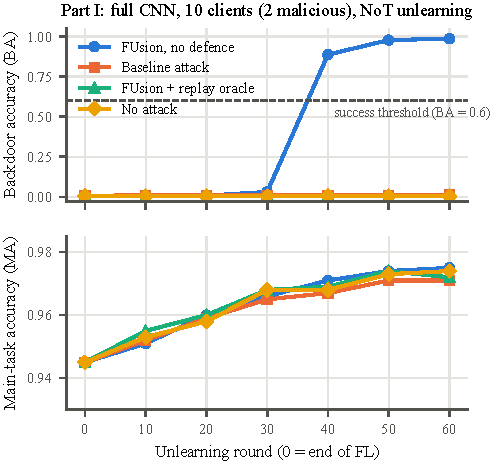
\includegraphics[width=\columnwidth]{figures/fig_part1.pdf}
\caption{Part I trajectories. FUsion stays dormant during FL and the first 30 unlearning rounds,
then crosses the success threshold between rounds 30 and 40. The replay oracle rejects all 120
patched updates, and \MA\ is unaffected in every run.}\label{fig:part1}
\end{figure}

\textbf{Results.} Table~\ref{tab:part1} and Fig.~\ref{fig:part1} summarise Part~I.
\begin{itemize}
\item \emph{The attack works.} The attackers localised the backdoor to a contiguous BC block
(conv2+fc1) with only 9 trigger-sensitive units. FUsion reached $\BA=0.986$ with \MA\ unchanged,
while the baseline attack (direct backdoor fine-tuning, no subnetwork) failed ($\BA=0.012$). This
reproduces the paper's central claim.
\item \emph{SubID detects it.} SubID found both attackers with TPR\,$=1$ and FPR\,$=0$, and raised
no false alarm without an attack.
\item \emph{The replay oracle blocks it.} The oracle rejected every patched update and kept
$\BA=0.005$. This motivates Part~II: obtain the same guarantee \emph{without} the server seeing the
data.
\end{itemize}

%=====================================================================
\section{Part II: Verifiable FL/FU Design}\label{sec:design}
%=====================================================================
This section restates the prevention mechanism of~\cite{zkdesign}, which we implement.

\subsection{Step 1: prove the procedure}
The server fixes the training procedure and writes it once as an arithmetic circuit. Every update,
FL or FU, must come with a proof that it is the output of that procedure, started from the global
model the server sent. A patched update $\hat w+\beta S_{bd}+\dots$ is not the output of the
procedure, so no valid proof for it exists. The ZK layer does not \emph{detect} the patch; it makes
the patch \emph{impossible to justify}.

\subsection{Step 2: bind the data}
A procedure-only proof is silent about which data went in. Before training, each client therefore
publishes $\mathrm{Com}(A)$, the root of a Merkle tree over its salted samples. This commitment
hides the data and locks it. Every later proof must open each sample it uses against
$\mathrm{Com}(A)$.

\subsection{Step 3: a bitmask instead of changing lists (from zkUnlearner~\cite{zkunlearner})}
Keeping changing lists of training and removed data would force a new circuit and a new setup for
each unlearning request. Instead, $A$ stays fixed and a bit $b_j$ marks each sample (1 = use,
0 = forget). Each sample's gradient is multiplied by its bit, which masks the \emph{data}, not the
weights. FL uses all-ones (except padding). An FU request sends $b$ in plain; the server validates
and stores it, and every later proof uses it. Forgotten data therefore never returns. Because only
the mask changes, $C_{\text{FL}}$ and $C_{\text{FU}}$ are fixed and need a single setup.

\subsection{What one proof binds}
\begin{enumerate}
\item \emph{Data:} the circuit re-hashes the batch samples and follows their Merkle paths to
$\mathrm{Com}(A)$, and the same values are then used for training.
\item \emph{Batch:} batch positions come from randomness tied to the model, the round and the
client, so the client cannot pick a convenient subset.
\item \emph{Mask:} the mask bits are public inputs.
\item \emph{Model:} the starting model must hash to the model the server sent, and the result must
hash to the update the client returned.
\item \emph{Replay:} the round and the client identifier are public inputs.
\end{enumerate}
The server sees only the public inputs and a 196-byte proof. Samples, salts, paths and
intermediate values stay with the client.

\subsection{Pipeline and random auditing}
\begin{enumerate}
\item \emph{Setup (once):} the server publishes the circuit and keys, and each client publishes
$\mathrm{Com}(A)$.
\item \emph{FL rounds:} the client sends an update with a proof, and the server verifies and
aggregates.
\item \emph{Unlearning request:} the client sends $b$, and the server checks and stores it.
\item \emph{FU rounds:} the same procedure with mask $b$; a patched update is rejected and the
client flagged.
\item \emph{After FU:} every later proof keeps using $b$.
\end{enumerate}
Proving dominates the cost, so~\cite{zkdesign} proposes \emph{random auditing}. After an update
arrives, the server requests its proof with probability $p$. A client that patches $m$ rounds
escapes only if none of them is audited, so
\begin{equation}
P(\text{caught})=1-(1-p)^m .\label{eq:audit}
\end{equation}
Auditing is safe only if (i) audits are unpredictable, i.e., decided after submission, and (ii)
clients keep each round's data so that they can prove later.

\begin{figure*}[t]
\centering
\resizebox{\textwidth}{!}{%
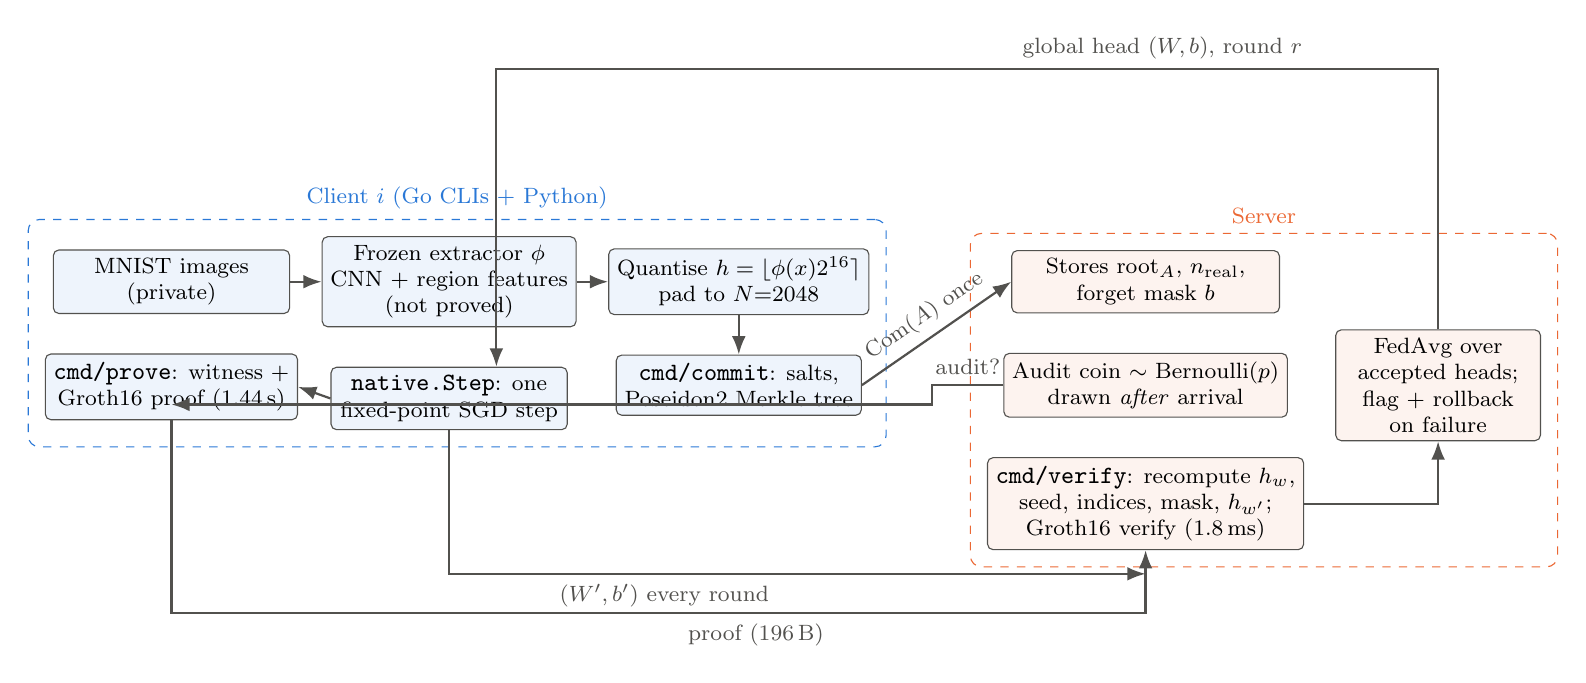
\begin{tikzpicture}[font=\footnotesize, >=Latex,
  box/.style={draw=cink, rounded corners=2pt, align=center, inner sep=3pt, minimum height=7mm},
  cl/.style={box, fill=cblue!8}, sv/.style={box, fill=corange!8}, ar/.style={->, thick, cink}]
\node[cl, minimum width=30mm] (img) {MNIST images\\ (private)};
\node[cl, right=4mm of img, minimum width=30mm] (ext) {Frozen extractor $\phi$\\ CNN + region features\\ (not proved)};
\node[cl, right=4mm of ext, minimum width=30mm] (q) {Quantise $h=\lfloor\phi(x)2^{16}\rceil$\\ pad to $N{=}2048$};
\node[cl, below=5mm of q, minimum width=30mm] (com) {\code{cmd/commit}: salts,\\ Poseidon2 Merkle tree};
\node[cl, below=5mm of ext, minimum width=30mm] (nat) {\code{native.Step}: one\\ fixed-point SGD step};
\node[cl, below=5mm of img, minimum width=30mm] (prv) {\code{cmd/prove}: witness +\\ Groth16 proof (1.44\,s)};
\node[fit=(img)(ext)(q)(com)(nat)(prv), draw=cblue, dashed, rounded corners, inner sep=6pt,
      label={[cblue]above:Client $i$ (Go CLIs + Python)}] (C) {};
\node[sv, right=18mm of q, minimum width=34mm] (st) {Stores $\mathrm{root}_A$, $n_{\text{real}}$,\\ forget mask $b$};
\node[sv, below=5mm of st, minimum width=34mm] (aud) {Audit coin $\sim$ Bernoulli($p$)\\ drawn \emph{after} arrival};
\node[sv, below=5mm of aud, minimum width=34mm] (ver) {\code{cmd/verify}: recompute $h_w$,\\ seed, indices, mask, $h_{w'}$;\\ Groth16 verify (1.8\,ms)};
\node[sv, right=6mm of aud, minimum width=26mm] (agg) {FedAvg over\\ accepted heads;\\ flag + rollback\\ on failure};
\node[fit=(st)(aud)(ver)(agg), draw=corange, dashed, rounded corners, inner sep=6pt,
      label={[corange]above:Server}] (S) {};
\draw[ar] (img) -- (ext); \draw[ar] (ext) -- (q); \draw[ar] (q) -- (com);
\draw[ar] (com.east) -- node[above, sloped]{$\mathrm{Com}(A)$ once} (st.west);
\draw[ar] (nat.west) -- (prv.east);
\draw[ar] (agg.north) |- node[above, pos=0.75]{global head $(W,b)$, round $r$} ([yshift=19mm]C.north east) -| ([xshift=6mm]nat.north);
\draw[ar] (nat.south) |- node[below, pos=0.7]{$(W',b')$ every round} ([yshift=-3mm]ver.south west) -- ([yshift=-3mm]ver.south);
\draw[ar] (aud.west) -- node[above]{audit?} ++(-9mm,0) |- ([yshift=2mm]prv.south) ;
\draw[ar] (prv.south) |- node[below, pos=0.8]{proof (196\,B)} ([yshift=-8mm]ver.south) -- (ver.south);
\draw[ar] (ver.east) -| (agg.south);
\end{tikzpicture}}
\caption{System overview. Clients commit once. Every round they compute the honest fixed-point
step natively and return the new head. The server decides \emph{after} receipt whether to audit;
an audited client rebuilds the witness deterministically and proves. The server recomputes every
public input itself, verifies, and aggregates only accepted heads, rolling back on a failed proof.}
\label{fig:arch}
\end{figure*}

%=====================================================================
\section{Why Groth16?}\label{sec:why}
%=====================================================================
Table~\ref{tab:ps} compares the proof systems we considered. The figures for systems other than
Groth16 are typical orders of magnitude from the literature, not our measurements, and they vary
with the implementation and the circuit.

\begin{table}[t]
\centering\footnotesize\caption{Proof-system comparison (typical orders of magnitude; Groth16 measured).}\label{tab:ps}
\setlength{\tabcolsep}{2.4pt}
\resizebox{\columnwidth}{!}{%
\begin{tabular}{@{}lcccc@{}}
\toprule
System & Setup & Proof size & Verify & Prover \\\midrule
\textbf{Groth16}~\cite{groth16} & per circuit & \textbf{196\,B (meas.)} & \textbf{1.8\,ms (meas.)} & fastest (R1CS) \\
PLONK~\cite{plonk} & universal & $\sim$0.5--1\,KB & ms & slower \\
Halo2 (IPA)~\cite{halo2} & none & few KB & tens of ms+ & slower \\
STARK~\cite{stark} & none & tens--100s KB & ms--tens ms & fast, big proofs \\
Bulletproofs~\cite{bulletproofs} & none & $\sim$1--2\,KB & linear (slow) & slow \\\bottomrule
\end{tabular}}
\end{table}

We chose Groth16 for five reasons.
\begin{enumerate}
\item \textbf{The server verifies many proofs every round.} With 50 clients, Groth16's constant
three-pairing check verifies a whole round in 0.116\,s (2.3\,ms per client, including recomputing
public inputs). Its constant 196-byte proof also adds negligible upload per client.
\item \textbf{The circuit never changes, so the per-circuit setup is paid once.} This is Groth16's
main drawback, but the bitmask design makes $C_{\text{FL}}=C_{\text{FU}}$ independent of rounds and
of unlearning requests. The setup took 16\,s, once, which is exactly the property the ZK design
targets.
\item \textbf{The workload is multiplication-heavy and maps naturally onto R1CS.} The step is
dominated by $2\times20\,480$ field multiplications and hashing, each multiplication being one R1CS
constraint. gnark's Groth16 prover is among the fastest available, and it supports
commitment-based log-derivative lookups~\cite{habock}, which make range checks cheap inside
Groth16.
\item \textbf{The tooling guarantees native/circuit agreement.} gnark~\cite{gnark} (Go) ships
matching native (gnark-crypto) and in-circuit implementations of Poseidon2, so the client's native
trainer and the circuit share one code base. This is what makes bit-identical updates achievable.
\item \textbf{It is comparable with prior work.} zkUnlearner~\cite{zkunlearner} and the cost table
of~\cite{zkdesign} both use Groth16 (192\,B proofs), so our measurements can be compared with
theirs directly.
\end{enumerate}
The trade-offs are a trusted setup (a deployment needs an MPC ceremony; our prototype uses a
single-party setup), no post-quantum security, and a new setup for any change to the circuit.

%=====================================================================
\section{Circuit Design}\label{sec:circuit}
%=====================================================================
\begin{table}[t]
\centering\footnotesize\caption{Protocol constants (single source: \code{params/params.go}).}\label{tab:params}
\begin{tabular}{@{}lll@{}}
\toprule
Symbol & Value & Meaning\\\midrule
$D,\ C$ & 64, 10 & head input and output size\\
$B$ & 32 & batch size of one proved step\\
$N$, depth & 2048, 11 & padded dataset size, Merkle depth\\
FRAC & 16 & fractional bits of the fixed-point encoding\\
$s$ & 8 & $\eta/B=2^{-s}$ (learning rate as a shift)\\
$k$ & 1 & SGD steps per round $=$ steps per proof\\
range & $[-2^{24},2^{24})$ & every private numeric value\\\bottomrule
\end{tabular}
\end{table}

\subsection{What is proved: a frozen extractor and a linear head}
Proving the whole CNN is out of reach. The second conv layer alone performs about $8.2\times10^5$
multiply-accumulates per sample in the forward pass. Over a batch of 32, forward and backward, that
is of the order of $10^8$ constraints, which means minutes to hours per proof and a proving key of
tens of GB. Following~\cite{zkdesign}, the convolutional extractor $\phi$ is pre-trained once on
\emph{public} data and frozen, and clients send only the head, so $\phi$ cannot be changed. The
proved model is the linear head $z=Wh+b$ with $W\in\mathbb{Z}^{10\times64}$.

\textbf{MSE loss, not cross-entropy.} Softmax needs $\exp$ and division, which in a circuit means
lookup tables or polynomial approximations. MSE against one-hot targets has the error
$e=z-y_{\text{onehot}}$ and gradients $\nabla_W=e\,h^\top$, all of them additions and
multiplications.

\textbf{Feature scaling.} The real update is $\Delta W=2^{-8}\sum_j m_je_jh_j^\top$, an effective
learning rate of 0.125. Stability requires $0.125\,\lambda_{\max}(\mathbb{E}[hh^\top])<2$. The
features are therefore centred by the public mean and L2-normalised to $\|h\|\approx2.5$.

\subsection{Fixed-point arithmetic and truncation}
A value $v$ is encoded as $\lfloor v\cdot2^{16}\rceil$; negative numbers become $p-|x|$ in the
field. Each dot product is accumulated at full precision and \emph{truncated once}:
$z_c=\mathrm{trunc}(\sum_dW_{cd}h_d,16)+b_c$. The gradients are
$G_W=\sum_jm_je_jh_j^\top$ and $G_b=\sum_jm_je_j$, and the update is
$W'=W-\mathrm{trunc}(G_W,24)$, $b'=b-\mathrm{trunc}(G_b,8)$. Dividing by the constant $B$ (inside
$s$), rather than by the number of unmasked samples, avoids any in-circuit division.

\textbf{Truncation gadget.} For signed $x$ with $|x|<2^{n-1}$, set $x'=x+2^{n-1}$. A hint supplies
$q,r$, and the circuit enforces
\begin{equation}
\begin{gathered}
x'=q\cdot2^t+r,\qquad 0\le r<2^t,\qquad 0\le q<2^{n-t},\\
\mathrm{trunc}(x,t)=q-2^{n-1-t}.
\end{gathered}
\end{equation}
Because $q2^t+r<2^n\ll p$, the decomposition is unique, so the hint is fully constrained. An
out-of-width $x$ has no witness at all. The native trainer performs the identical computation.

\textbf{Bound derivation} (Table~\ref{tab:bounds}). With $|W|,|h|,|b|\le2^{24}$, we size each
truncation to the worst case. All intermediates stay far below $p/2$, so the signed encoding is
unambiguous.

\begin{table}[t]
\centering\footnotesize\caption{Worst-case bounds and truncation widths.}\label{tab:bounds}
\setlength{\tabcolsep}{3pt}
\resizebox{\columnwidth}{!}{%
\begin{tabular}{@{}llc@{}}
\toprule
Quantity & Bound & Width $n$ (bits of $q$) \\\midrule
$\sum_{d<64}W h$ & $64\cdot2^{48}=2^{54}$ & 56 (40) for $\mathrm{trunc}(\cdot,16)$\\
$e=z-y$ & $<2^{39}$ & --\\
$G_W=\sum_{j<32}m e h$ & $32\cdot2^{39}\cdot2^{24}=2^{68}$ & 70 (46) for $\mathrm{trunc}(\cdot,24)$\\
$G_b=\sum_{j<32}m e$ & $2^{44}$ & 46 (38) for $\mathrm{trunc}(\cdot,8)$\\
$W'$ & $<2^{45}$ & range-checked to $[-2^{24},2^{24})$\\\bottomrule
\end{tabular}}
\end{table}

\subsection{Range checks: defeating field wrap-around}
Without range checks, a prover could pass $p-2^{40}$ as a ``small negative'' feature, or exploit
wrap-around in the multiplications. Every private numeric witness is therefore range-checked:
features, labels (through a one-hot whose entries must sum to 1), $W$, $b$, and also $W'$, $b'$.
gnark implements these checks with log-derivative lookups~\cite{habock} backed by a commitment
inside Groth16. A complete truncation, including its two range checks, costs only 18--25
constraints at the margin. The soundness tests include out-of-range and wrapped values, each with
an in-range control.

\subsection{Hashing: Poseidon2, with packing}
The leaves, the Merkle nodes and the head digests all use one hash $H$, Merkle--Damg\aa rd over the
Poseidon2~\cite{poseidon2} width-2 compression with IV 0. The native and in-circuit versions come
from the same gnark release and are tested to agree. Fig.~\ref{fig:hash} shows the measured costs:
a 2-to-1 Poseidon2 hash costs 372 constraints, against 661 for MiMC~\cite{mimc} and 68\,411 for
SHA-256. With SHA-256 the circuit would exceed 40\,M constraints.

To cut hashing further, each range-checked 25-bit value $u=v+2^{24}$ is packed nine to a field
element ($225<253$ bits). A leaf then costs 10 absorbs instead of 66, and a head digest 73 instead
of 650. Packing is a linear combination, which is free in R1CS, and it is injective \emph{only}
because every packed value is range-checked. This is why the circuit also range-checks $W'$, $b'$,
an addition to the original specification. Packing shrinks the circuit from about 0.75\,M to
0.29\,M constraints.

\begin{figure}[t]
\centering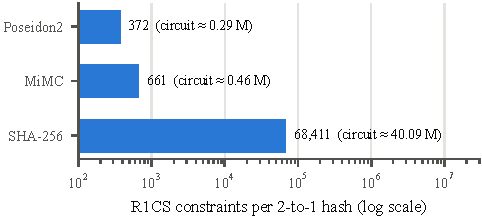
\includegraphics[width=\columnwidth]{figures/fig_hash.pdf}
\caption{Measured R1CS cost of one 2-to-1 hash in gnark v0.16.5, and the projected size of our
circuit with each hash.}\label{fig:hash}
\end{figure}

\subsection{Commitment, indices and public inputs}
Leaf $i$ is $H(\text{salt}_i,P_0,\dots,P_7,y_i)$, where $P_k$ are the packed features, and a Merkle
node is $H(\ell,r)$. Padding samples ($i\ge n_{\text{real}}$) have zero features and their mask bit
is forced to 0. The server derives $\text{seed}=H(h_w,r,\text{id})$ and
$\text{idx}_j=H(\text{seed},j)\bmod2^{11}$, sampling with replacement, so duplicates are allowed.
The 11 bits of $\text{idx}_j$, unpacked in-circuit, are \emph{the} Merkle direction bits; a sample
can therefore only be opened at its committed position.

There are 8 public inputs, kept small because Groth16 verification costs one scalar multiplication
per input: $\mathrm{root}_A$, $h_w$, $h_{w'}$, two packed index words (16$\times$11 bits each), one
packed mask word (32 bits), the round and the client identifier. The round and the client
identifier are bound by one constraint, $(r+1)(\text{id}+1)=t$. A public input that appears in no
constraint has a zero verification-key term and could be swapped freely.

\begin{figure}[t]
\centering
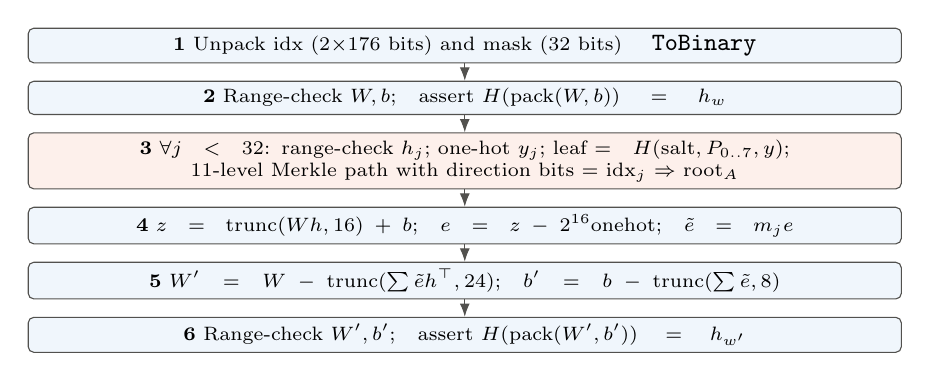
\begin{tikzpicture}[font=\scriptsize, >=Latex, node distance=2.2mm,
  st/.style={draw=cink, rounded corners=2pt, fill=cblue!7, align=center, text width=0.9\columnwidth, inner sep=2.5pt}]
\node[st] (a) {\textbf{1} Unpack idx (2$\times$176 bits) and mask (32 bits) \quad\code{ToBinary}};
\node[st, below=of a] (b) {\textbf{2} Range-check $W,b$;\quad assert $H(\mathrm{pack}(W,b))=h_w$};
\node[st, below=of b, fill=corange!10] (c) {\textbf{3} $\forall j<32$: range-check $h_j$; one-hot $y_j$; leaf $=H(\text{salt},P_{0..7},y)$;\\ 11-level Merkle path with direction bits $=$ idx$_j$ $\Rightarrow$ $\mathrm{root}_A$};
\node[st, below=of c] (d) {\textbf{4} $z=\mathrm{trunc}(Wh,16)+b$;\quad $e=z-2^{16}\mathrm{onehot}$;\quad $\tilde e=m_j e$};
\node[st, below=of d] (e) {\textbf{5} $W'=W-\mathrm{trunc}(\sum\tilde e h^\top,24)$;\quad $b'=b-\mathrm{trunc}(\sum\tilde e,8)$};
\node[st, below=of e] (f) {\textbf{6} Range-check $W',b'$;\quad assert $H(\mathrm{pack}(W',b'))=h_{w'}$};
\foreach \x/\y in {a/b,b/c,c/d,d/e,e/f} \draw[->, cink] (\x) -- (\y);
\end{tikzpicture}
\caption{Constraint flow of \code{ZkStepCircuit}. The same $h_j,y_j$ wires feed the Merkle check
(step 3) and the training step (steps 4--5), so the data checked is exactly the data trained on.}
\label{fig:circuit}
\end{figure}

\begin{figure}[t]
\centering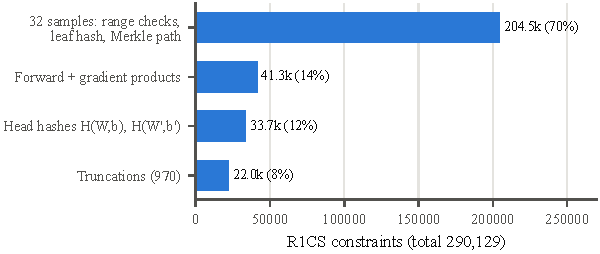
\includegraphics[width=\columnwidth]{figures/fig_constraints.pdf}
\caption{Constraint breakdown (marginal costs). Merkle paths over the 32 sampled leaves dominate;
the training arithmetic is about 22\,\%. Lookup amortisation in the full circuit accounts for the
remaining $-11$k.}\label{fig:constraints}
\end{figure}

%=====================================================================
\section{Implementation}\label{sec:impl}
%=====================================================================
\textbf{Stack.} The cryptographic core is in Go~1.26 with gnark v0.16.5 (Groth16, BN254, R1CS) and
gnark-crypto (native Poseidon2). The orchestration, MNIST loading, the extractor and the attacker
are in Python 3.12 with PyTorch 2.15. Python \emph{never} computes an honest weight update: every
honest step comes from the Go native trainer, which is what makes native and proved updates
bit-identical. The packages are \code{params} (one constants file), \code{native} (reference
trainer), \code{commit} (hash, packing, Merkle tree, private dataset files), \code{circuit}
(gadgets, \code{ZkStepCircuit}), \code{protocol} (seed, indices, mask, public inputs, key and proof
I/O), CLIs \code{setup}, \code{commit}, \code{prove}, \code{verify}, \code{bench} and
\code{hashcost} with JSON input and output, and \code{sim} (Python).

\textbf{Server logic.}
\begin{itemize}
\item The server recomputes every public input from its own state; the client supplies only the
returned head and the proof.
\item Heads outside the value range are rejected before hashing.
\item An unlearning request must lie within $[0,N)$, include at least one non-padding position,
and may only clear bits.
\item Aggregation is exact-integer FedAvg with deterministic re-quantisation,
$\lfloor(\Sigma+\lfloor n/2\rfloor)/n\rfloor$, clipped to the value range.
\end{itemize}

\textbf{Auditing.} The audit coin comes from a server-only RNG, drawn after an update arrives.
Because the procedure is deterministic, an audited client rebuilds the exact witness from the
round's stored inputs (global head, round, mask). A failed proof flags the client and excludes it
from then on. During FU, the default \emph{rollback} policy also reverts the global model to the
FU-start checkpoint, since un-audited patched updates may already have been aggregated. This
mirrors SubID's ``discard and retrain''. The \emph{exclude} policy is reported for comparison.

\textbf{Attacker.} FUsion is adapted to the head-only model, keeping the paper's hyperparameters
($\beta=0.2$, $\rho=0.1$, $\lambda=0.5$):
\begin{itemize}
\item the head is the only BC layer;
\item TS units are the head's input dimensions, ranked by the Grad-CAM score
$\mathrm{relu}(W^{bd}_{t,d}h_d)$;
\item the subnetwork trains $W[:,\text{TS}]$ with the clean-logit regulariser of Eq.~(10);
\item each FU round, the attacker takes the honest Go step, fuses $\beta S_{bd}$, fine-tunes on
clean plus backdoor data, and quantises.
\end{itemize}

\textbf{Extractor variants.} A purely clean-pretrained CNN discards the 3$\times$3 corner trigger:
even a head trained on 10\,\% poisoned data reaches only $\BA\approx0.01$ (an 8$\times$8 trigger
reaches 0.09). The main experiments therefore use 48 CNN features plus 16 fixed region intensities
(the mean of each $7\times7$ cell). A poisoned head then reaches $\BA=0.82$, so the defence is
evaluated against an attack that actually works. The pure-CNN variant is reported as an ablation.

\textbf{Correctness evidence} (\code{go test}, 55\,s, all pass):
\begin{itemize}
\item truncation gadget vs.\ native truncation vs.\ floor division on random, zero, $\pm1$,
$\pm2^t\pm1$ and both width extremes;
\item Poseidon2 native vs.\ library vs.\ circuit for every input length used;
\item Merkle native vs.\ circuit;
\item \textbf{1000/1000 random steps bit-identical} between native and circuit (four feature
scales, four weight scales, FL and FU masks);
\item completeness for honest FL and FU steps;
\item soundness: rejection of every case in Table~\ref{tab:sound}.
\end{itemize}

\begin{table}[t]
\centering\footnotesize\caption{Soundness tests: every manipulation is rejected.}\label{tab:sound}
\setlength{\tabcolsep}{3pt}
\resizebox{\columnwidth}{!}{%
\begin{tabular}{@{}ll@{}}
\toprule
Manipulation & How it fails\\\midrule
One weight $+1$ unit (backdoor patch) & verify rejects; no witness\\
Wrong starting model & no witness; proof rejected\\
Fresh sample / modified feature / label & Merkle check fails\\
Committed sample at another index & direction bits mismatch\\
Forgotten sample's mask bit $0\to1$ & proof rejected (server's mask)\\
Proof replayed across clients or rounds & verify rejects\\
Only round, or only client id changed & verify rejects (binding)\\
Out-of-range feature (in-range control passes) & range check fails\\
Out-of-range weight, wrapped feature, label $=10$ & range / one-hot fails\\\bottomrule
\end{tabular}}
\end{table}

%=====================================================================
\section{Evaluation}\label{sec:eval}
%=====================================================================
\textbf{Setup.}
\begin{itemize}
\item \emph{Hardware:} Apple M3 (8 cores, 16\,GB), CPU only.
\item \emph{Federation:} 50 clients with 1\,000 IID MNIST samples each; the extractor is
pre-trained on the other 10\,000 training images (public); 10 clients are malicious (20\,\%) and 5
benign clients also request unlearning, forgetting 2\,\% of their data.
\item \emph{Schedule:} 20 FL rounds, then 20 FU rounds. These defaults keep each run to minutes.
\item \emph{Runs:} one seed per configuration; Table~\ref{tab:analytic} gives the analytic
probabilities that the audit outcomes should be read against.
\item \emph{Reproduction:} \code{zkfu/run\_experiments.sh} produces every number, and
\code{make\_figures.py} draws every figure from the raw JSON.
\end{itemize}

\subsection{Cost of every step}
\begin{table}[t]
\centering\footnotesize\caption{Time of every important step (measured).}\label{tab:steps}
\setlength{\tabcolsep}{3pt}
\resizebox{\columnwidth}{!}{%
\begin{tabular}{@{}llr@{}}
\toprule
Phase & Step & Time \\\midrule
\multirow{5}{*}{\shortstack[l]{One-time}} & Pre-train extractor (10k public images) & 2.12\,s\\
 & Extract features (50k images) & 1.25\,s\\
 & Compile circuit (290\,129 constraints) & 0.34\,s\\
 & Groth16 setup (peak RAM 0.60\,GB) & 16.0\,s\\
 & Commit one client / all 50 clients & 112\,ms / 7.3\,s\\\midrule
\multirow{4}{*}{\shortstack[l]{Client,\\every round}} & Native fixed-point step & 1.48\,ms\\
 & 50-client native round (incl.\ I/O) & 147\,ms\\
 & Attacker patch (fuse + fine-tune) & 8.1\,ms\\
 & Load proving key (117\,MB, raw) & 0.10\,s\\\midrule
\multirow{3}{*}{\shortstack[l]{Client,\\when proving}} & Merkle tree rebuild (2048 leaves) & 109\,ms\\
 & Witness assembly & 0.37\,ms\\
 & \textbf{Groth16 proof} (peak RAM 0.93\,GB) & \textbf{1.44$\pm$0.06\,s}\\\midrule
\multirow{3}{*}{Server} & \textbf{Verify one proof} & \textbf{1.83\,ms}\\
 & Verify 50 proofs incl.\ public inputs & 0.116\,s\\
 & Full round (I/O + verify 50 + FedAvg) & 0.33\,s\\\bottomrule
\end{tabular}}
\end{table}

\begin{figure}[t]
\centering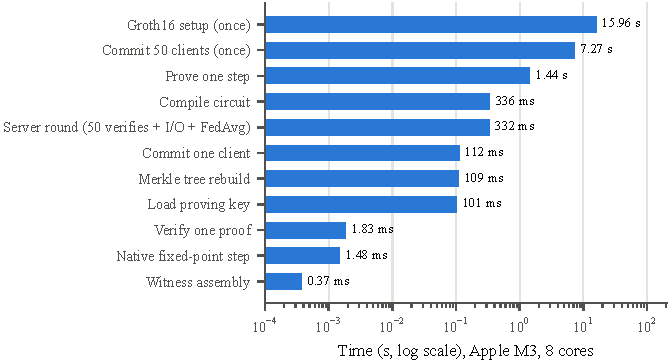
\includegraphics[width=\columnwidth]{figures/fig_timing.pdf}
\caption{Step times on a log scale. Proving is about 1\,000$\times$ the plain step and dominates;
verification is three orders of magnitude cheaper than proving.}\label{fig:timing}
\end{figure}

Table~\ref{tab:steps} and Fig.~\ref{fig:timing} give the cost of every step. Over 20 consecutive
real training steps the proving time was $1.439\pm0.061$\,s (min 1.38\,s, max 1.65\,s), with
proofs of 196\,B (128\,B for Groth16 itself plus gnark's range-check commitment). Table~\ref{tab:est}
compares these measurements with the design's estimates.

\begin{table}[t]
\centering\footnotesize\caption{Measured vs.\ the ZK design's estimates~\cite{zkdesign}.}\label{tab:est}
\setlength{\tabcolsep}{3pt}
\begin{tabular}{@{}lcc@{}}
\toprule
Item & Estimate & Measured \\\midrule
Proof, MNIST head, per step & 2--10\,s & \textbf{1.44\,s}\\
Verification & 0.2\,s & \textbf{1.8\,ms}\\
Proof size & 192\,B & 196\,B\\
Server, 50 clients, per round & $<10$\,s & \textbf{0.12\,s}\\
Proving per client, 500 FL + 200 FU & 1--2\,h & \textbf{$\approx$18\,min}\\\bottomrule
\end{tabular}
\end{table}

\subsection{Accuracy cost of fixed point}
We trained the same head in floating point under the identical schedule and update rule. It reached
\MA\ 0.9379 after FL and 0.9452 after FU, against 0.9345 and 0.9454 for the proved fixed-point head
(Fig.~\ref{fig:ma}). The cost is at most 0.34 percentage points and vanishes after FU.

\begin{figure}[t]
\centering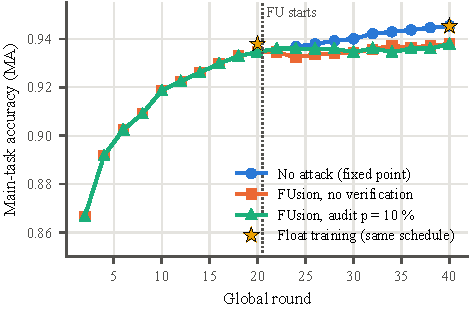
\includegraphics[width=\columnwidth]{figures/fig_part2_ma.pdf}
\caption{Main-task accuracy over all 40 rounds. Fixed point tracks float training (stars). The
attacked runs keep \MA\ intact, so FUsion is stealthy here as well.}\label{fig:ma}
\end{figure}

\subsection{Attack vs.\ defence}
\begin{table*}[t]
\centering\footnotesize\caption{Attack vs.\ defence, 50 clients (10 malicious), 20 FL + 20 FU rounds. ``Proving
time'' is the sum over all proofs (each uses 8 cores); clients would prove in parallel.}\label{tab:main}
\setlength{\tabcolsep}{3.2pt}
\begin{tabular}{@{}llccccccrrr@{}}
\toprule
Run & Verification & \MA\ (FL end) & \MA\ (final) & \BA\ (final) & Attack & Caught & FP & Rollbacks & Proofs & Proving time\\\midrule
E1 & none, no attack & 0.934 & 0.945 & 0.011 & -- & -- & 0 & 0 & 0 & 0\\
\textbf{E0} & \textbf{none} & 0.934 & 0.938 & \textbf{1.000} & \textbf{yes} & 0/10 & 0 & 0 & 0 & 0\\
\textbf{F} & \textbf{every update ($p=1$)}$^\dagger$ & 0.934 & 0.937 & \textbf{0.013} & no & \textbf{10/10 (rd.\,1)} & 0 & 1 & 130 & 203\,s\\
A05 & audit $p=5\,\%$, rollback & 0.934 & 0.937 & 0.034 & no & 7/10 & 0 & 4 & 97 & 155\,s\\
A10 & audit $p=10\,\%$, rollback & 0.934 & 0.938 & 0.019 & no & 9/10 & 0 & 6 & 186 & 318\,s\\
A20 & audit $p=20\,\%$, rollback & 0.934 & 0.941 & 0.013 & no & 10/10 & 0 & 5 & 363 & 619\,s\\
A10x & audit $p=10\,\%$, \textbf{exclude only} & 0.934 & 0.942 & \textbf{0.789} & \textbf{yes} & 9/10 & 0 & 0 & 186 & 308\,s\\
E2 & none, pure-CNN extractor & 0.945 & 0.892 & 0.077 & no & -- & 0 & 0 & 0 & 0\\\bottomrule
\multicolumn{11}{@{}p{0.97\textwidth}@{}}{$^\dagger$F resumes from E0's FL-final model and runs 3 FU rounds with all 50 clients proving; the full-schedule cost is extrapolated in Table~\ref{tab:cost}.}
\end{tabular}
\end{table*}

\begin{figure*}[t]
\centering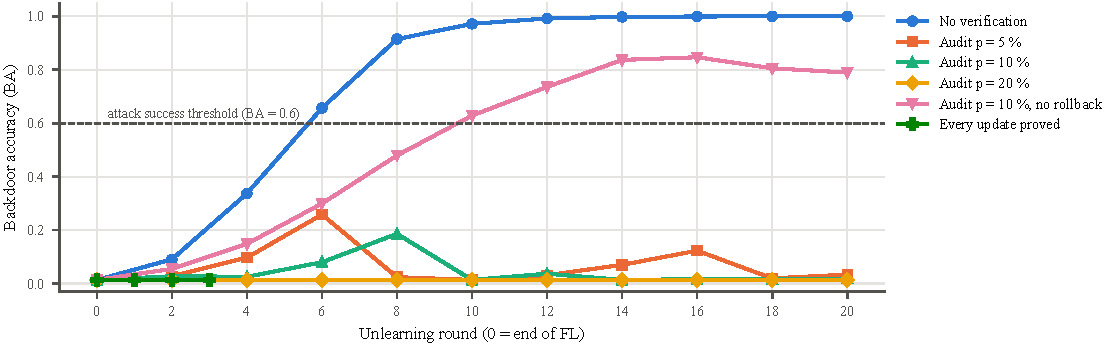
\includegraphics[width=\textwidth]{figures/fig_part2_ba.pdf}
\caption{Backdoor accuracy during unlearning. Without verification FUsion passes $\BA=0.6$ after 6
rounds and reaches 1.0. Proving every update keeps \BA\ at baseline. Auditing with rollback ends at
baseline for every $p$, with transient peaks (0.26 at $p=5\,\%$, 0.19 at $p=10\,\%$) before each
catch. With the \emph{same} audit draws but no rollback, the uncaught attacker drives \BA\ to
0.79.}\label{fig:ba}
\end{figure*}

Table~\ref{tab:main} and Fig.~\ref{fig:ba} give the outcomes.
\begin{itemize}
\item \textbf{No verification (E0).} FUsion takes \BA\ from 0.011 to 1.000 while \MA\ stays at
0.938. It needs $m=6$ patched rounds to pass $\BA=0.6$.
\item \textbf{Every update proved (F).} All 10 attackers fail verification the first time they
patch, \BA\ never moves, and none of the honest proofs is rejected. This is the deterministic
guarantee of~\cite{zkdesign}.
\item \textbf{Auditing with rollback (A05, A10, A20).} The final \BA\ is at baseline for every
$p$.
\item \textbf{Auditing without rollback (A10x).} With identical audit coins to A10, the attack
\emph{succeeds}: before its first audit, each attacker's patched updates were already aggregated,
and excluding the caught clients does not remove them.
\end{itemize}
Fig.~\ref{fig:catch} shows when each attacker was caught.

\begin{figure}[t]
\centering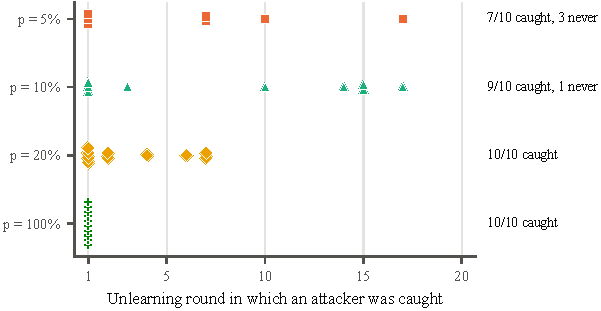
\includegraphics[width=\columnwidth]{figures/fig_catch.pdf}
\caption{Unlearning round in which each attacker was caught. Full proving catches all 10 at once.
Lower $p$ spreads catches over the FU phase, and some attackers are never audited.}\label{fig:catch}
\end{figure}

\subsection{Random auditing: security vs.\ cost}
\begin{figure*}[t]
\centering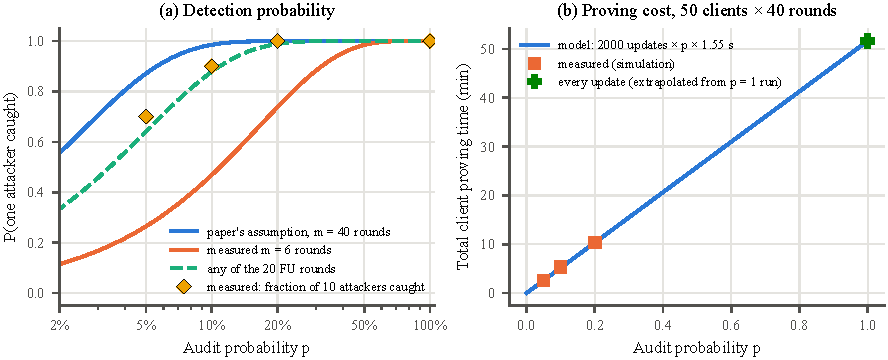
\includegraphics[width=\textwidth]{figures/fig_audit.pdf}
\caption{(a) Probability that a given attacker is caught, Eq.~(\ref{eq:audit}), with the design's
assumed $m=40$ and our measured $m=6$; measured catch fractions follow the 20-round curve. (b)
Total proving cost grows linearly in $p$; measured runs match the model.}\label{fig:audit}
\end{figure*}

\begin{table}[t]
\centering\footnotesize\caption{Eq.~(\ref{eq:audit}) with the measured $m=6$ vs.\ the assumed $m=40$.}\label{tab:analytic}
\setlength{\tabcolsep}{2.6pt}
\resizebox{\columnwidth}{!}{%
\begin{tabular}{@{}lccccc@{}}
\toprule
$p$ & $m=6$ & $m=40$ & 20 rounds & all 10, 20 rds & saved\\\midrule
5\,\% & 0.265 & 0.871 & 0.642 & 0.012 & 95\,\%\\
10\,\% & 0.469 & 0.985 & 0.878 & 0.274 & 90\,\%\\
20\,\% & 0.738 & 1.000 & 0.988 & 0.891 & 80\,\%\\
60\,\% & 0.996 & 1.000 & 1.000 & 1.000 & 40\,\%\\\bottomrule
\end{tabular}}
\end{table}

\begin{table}[t]
\centering\footnotesize\caption{Proving cost over the whole 40-round, 50-client schedule.}\label{tab:cost}
\setlength{\tabcolsep}{3pt}
\begin{tabular}{@{}lrrr@{}}
\toprule
Mode & Proofs & Total & Per client\\\midrule
Every update (extrapolated) & 2\,000 & 51.6\,min & 62\,s\\
Audit $p=5\,\%$ (measured) & 97 & 2.6\,min & 3\,s\\
Audit $p=10\,\%$ (measured) & 186 & 5.3\,min & 6\,s\\
Audit $p=20\,\%$ (measured) & 363 & 10.3\,min & 12\,s\\\bottomrule
\end{tabular}
\end{table}

The design~\cite{zkdesign} reads $m\approx40$ from one plot of~\cite{fusion}. In our setting $m=6$,
so the chance of catching a given attacker within its attack window drops sharply
(Table~\ref{tab:analytic}, Fig.~\ref{fig:audit}a). At $p=10\,\%$ it is 0.469, not 0.985. The
measured catch fractions (7/10, 9/10 and 10/10) agree with the 20-round column. Auditing still
prevented the backdoor because rollback resets the attackers' progress at every catch, and the
remaining few attackers need many uninterrupted rounds. The cost (Table~\ref{tab:cost},
Fig.~\ref{fig:audit}b) scales linearly in $p$: auditing at 10\,\% cuts total proving from 51.6 to
5.3\,min.

\subsection{Comparison of defences}
\begin{table*}[t]
\centering\footnotesize\caption{Defences against FUsion across both parts. Part I uses a full CNN with 10
clients and Part II a proved linear head with 50 clients, so \BA\ figures are not from the same
model.}\label{tab:compare}
\setlength{\tabcolsep}{4pt}
\begin{tabular}{@{}>{\raggedright\arraybackslash}p{3.5cm}>{\raggedright\arraybackslash}p{2.4cm}>{\raggedright\arraybackslash}p{1.1cm}>{\raggedright\arraybackslash}p{2.6cm}>{\raggedright\arraybackslash}p{3.5cm}>{\raggedright\arraybackslash}p{3.3cm}@{}}
\toprule
Defence & Kind & Data private & Guarantee & Outcome vs.\ FUsion & Cost\\\midrule
None (Part I / Part II) & -- & yes & none & \BA\ 0.986 / 1.000 & --\\
SubID~\cite{fusion} (Part I) & statistical detection & yes & empirical; needs a benign majority & 2/2 flagged, $F_1=1$; discard and retrain & SVD per window (negligible)\\
Replay oracle (Part I) & recomputation in the clear & \textbf{no} & deterministic & \BA\ 0.005, 120/120 patched rejected & server sees all data\\
\textbf{Groth16, every update} (Part II) & cryptographic & \textbf{yes} & \textbf{deterministic} & \textbf{\BA\ 0.013, 10/10 at first patch} & 1.44\,s/client/round; 0.12\,s/server/round\\
Groth16 + audit 10\,\%, rollback (Part II) & cryptographic & yes & probabilistic, Eq.~(\ref{eq:audit}) & \BA\ 0.019 (peak 0.19), 9/10 caught & $-90\,\%$ proving\\
Groth16 + audit 10\,\%, exclude (Part II) & cryptographic & yes & insufficient & \BA\ 0.789 (attack succeeds) & $-90\,\%$ proving\\\bottomrule
\end{tabular}
\end{table*}

Table~\ref{tab:compare} puts all defences side by side. Groth16 matches the outcome of the replay
oracle while keeping data private. Unlike SubID, it does not depend on attackers being a
statistical minority, and its decision is cryptographic rather than threshold-based.
Table~\ref{tab:related} positions the design against related approaches, following~\cite{zkdesign}.

\begin{table}[t]
\centering\footnotesize\caption{Related approaches (after~\cite{zkdesign}).}\label{tab:related}
\setlength{\tabcolsep}{2.5pt}
\resizebox{\columnwidth}{!}{%
\begin{tabular}{@{}p{2.15cm}p{2.7cm}p{3.1cm}@{}}
\toprule
Method & Verifies via & Difference from this design\\\midrule
VeriFi~\cite{verifi} & marker samples & statistical; checks effect, not procedure\\
zk-APEX~\cite{zkapex} & Halo2, one-shot step & masks weights; no data link; no per-round FL proofs\\
Membership lists & hashed lists + retraining proof & new circuit/setup per request\\
SubID~\cite{fusion} & update directions & statistical, not cryptographic\\
zkUnlearner~\cite{zkunlearner} & Groth16, bitmask & centralised trainer; one retraining\\
\textbf{This work} & Groth16 per FL/FU step & every round, committed data, fixed circuit\\\bottomrule
\end{tabular}}
\end{table}

%=====================================================================
\section{Discussion}\label{sec:discussion}
%=====================================================================
\textbf{Finding 1: auditing needs rollback.} A detected cheat must invalidate the model state that
may contain its earlier, un-audited patches. Excluding the client alone is not enough (A10x). The
design~\cite{zkdesign} should make rollback part of the protocol.

\textbf{Finding 2: $m$ can be small.} With $m=6$, the guarantee of Eq.~(\ref{eq:audit}) is far
weaker than the design's table suggests, and auditing leaves windows in which the model is
partially backdoored (peak \BA\ 0.26 at $p=5\,\%$). We recommend proving \emph{every FU round},
which is the only phase FUsion uses, and auditing only FL rounds. That is about 52\,\% of the full
cost in our schedule and about 32\,\% in the design's 500+200 schedule (with $p=5\,\%$ in FL), for
a deterministic guarantee exactly where the attack operates.

\textbf{Finding 3: the frozen extractor is itself a mitigation.} When the proved part is a linear
head on a clean-pretrained extractor, FUsion's capacity is limited by what the frozen features
retain. With pure CNN features the attack barely works even without proofs (E2: \BA\ 0.077, \MA\
$-5$ points). The added value of the ZK layer grows with the backdoor capacity of the proved
component.

\textbf{Limitations.}
\begin{itemize}
\item The setup is single-party; a deployment needs an MPC ceremony.
\item Aggregation and the extractor are not proved.
\item Poison committed from the start is data poisoning and is not prevented.
\item The plain mask reveals which positions are forgotten, and clients choose which samples to
forget.
\item Results use one seed per configuration.
\item Our deviations from the specification are documented: packed hash inputs, the extra
$W',b'$ range check, the interval $[-2^{24},2^{24})$, and the region-feature extractor.
\end{itemize}

%=====================================================================
\section{Conclusion}
%=====================================================================
We reproduced the FUsion backdoor and the SubID defence, then built and measured the
zero-knowledge prevention for active federated unlearning. A Groth16 proof of one fixed-point step
of a linear head, bound to a Poseidon2-Merkle-committed dataset and a public forget bitmask, costs
1.44\,s to produce and 1.8\,ms to verify, and makes FUsion's patched updates unprovable. Every
attacker is rejected at its first patch, with no accuracy cost relative to float training. Random
auditing reduces proving by up to 95\,\% but is only safe with rollback, and its probabilistic
guarantee depends on how many rounds the attack needs. Here that number was 6, not 40.

\section*{Reproducibility}
All code, raw results and figure scripts are in the project directory. Run
\code{zkfu/run\_experiments.sh} (about 30\,min), then \code{.venv/bin/python make\_figures.py},
then \code{go test ./tests/}. Commands are in \code{commands.md}; design notes are in
\code{zkfu/DESIGN\_NOTES.md}.

\begin{thebibliography}{99}
\bibitem{fusion} W.~Zhao, Y.~Peng, X.~Li, J.~Xu, Y.~Liu, and Z.~Lu, ``Malicious forgetting: Backdoor injection in active federated unlearning and countermeasure design,'' in \emph{Proc.\ IEEE INFOCOM}, 2026.
\bibitem{zkdesign} ``Verifiable federated unlearning with zero-knowledge proofs,'' design document (project reference), 2026.
\bibitem{zkunlearner} Wang \emph{et~al.}, ``zkUnlearner: A zero-knowledge framework for verifiable unlearning with multi-granularity and forgery-resistance,'' arXiv, 2025.
\bibitem{groth16} J.~Groth, ``On the size of pairing-based non-interactive arguments,'' in \emph{Proc.\ EUROCRYPT}, 2016.
\bibitem{gnark} Consensys, ``gnark: a zk-SNARK library,'' v0.16.5, \url{https://github.com/Consensys/gnark}.
\bibitem{poseidon2} L.~Grassi, D.~Khovratovich, and M.~Schofnegger, ``Poseidon2: A faster version of the Poseidon hash function,'' in \emph{Proc.\ AFRICACRYPT}, 2023.
\bibitem{mimc} M.~Albrecht \emph{et~al.}, ``MiMC: Efficient encryption and cryptographic hashing with minimal multiplicative complexity,'' in \emph{Proc.\ ASIACRYPT}, 2016.
\bibitem{habock} U.~Hab\"ock, ``Multivariate lookups based on logarithmic derivatives,'' IACR ePrint 2022/1530.
\bibitem{plonk} A.~Gabizon, Z.~Williamson, and O.~Ciobotaru, ``PLONK: Permutations over Lagrange-bases for oecumenical noninteractive arguments of knowledge,'' IACR ePrint 2019/953.
\bibitem{halo2} S.~Bowe, J.~Grigg, and D.~Hopwood, ``Recursive proof composition without a trusted setup,'' IACR ePrint 2019/1021.
\bibitem{stark} E.~Ben-Sasson, I.~Bentov, Y.~Horesh, and M.~Riabzev, ``Scalable, transparent, and post-quantum secure computational integrity,'' IACR ePrint 2018/046.
\bibitem{bulletproofs} B.~B\"unz \emph{et~al.}, ``Bulletproofs: Short proofs for confidential transactions and more,'' in \emph{Proc.\ IEEE S\&P}, 2018.
\bibitem{fedavg} B.~McMahan, E.~Moore, D.~Ramage, S.~Hampson, and B.~A.~y~Arcas, ``Communication-efficient learning of deep networks from decentralized data,'' in \emph{Proc.\ AISTATS}, 2017.
\bibitem{not} Y.~H.~Khalil \emph{et~al.}, ``NoT: Federated unlearning via weight negation,'' in \emph{Proc.\ CVPR}, 2025.
\bibitem{gradcam} R.~R.~Selvaraju \emph{et~al.}, ``Grad-CAM: Visual explanations from deep networks via gradient-based localization,'' in \emph{Proc.\ ICCV}, 2017.
\bibitem{verifi} X.~Gao \emph{et~al.}, ``VeriFi: Towards verifiable federated unlearning,'' \emph{IEEE TDSC}, 2024.
\bibitem{zkapex} Maheri \emph{et~al.}, ``ZK-APEX: Zero-knowledge approximate personalized unlearning with executable proofs,'' in \emph{Proc.\ MLSys}, 2026.
\bibitem{gdpr} European Parliament and Council, ``General Data Protection Regulation (EU) 2016/679,'' Art.~17, 2016.
\end{thebibliography}

\end{document}
